In this paper we shall explore sequences of billiard ball collisions. In particular, we look at the sequence of sides that a billiard ball collides with under perfect, frictionless conditions. We will show how a square billiards table can be analyzed by tiling the table in the plane, and prove a number of properties that billiard ball sequences must satisfy.

\section{Setup}

We will imagine an infinitesimally small billiard ball on a square table. For simplicity, we will assume that the square table is defined on the unit square, i.e. $[0,1]^2$. The ball will start at some initial position $\bvec{x}_0$ inside of the table and with some velocity $\bvec{v}_0$. We will assume that the ball is massless and frictionless, and that there is no gravity.

We will assume ideal, elastic collisions so that the ball conserves both kinetic energy and momentum when it hits a wall. To be more precise, when the ball collides with an edge of the table, the ball's velocity will be reflected across the line perpendicular to the edge of the table at the point of collision. In other words, the angle of the incoming velocity will be the same as the outgoing velocity. Figure \ref{fig:collision-angle} shows the general mechanics of a collision.

\begin{figure}
  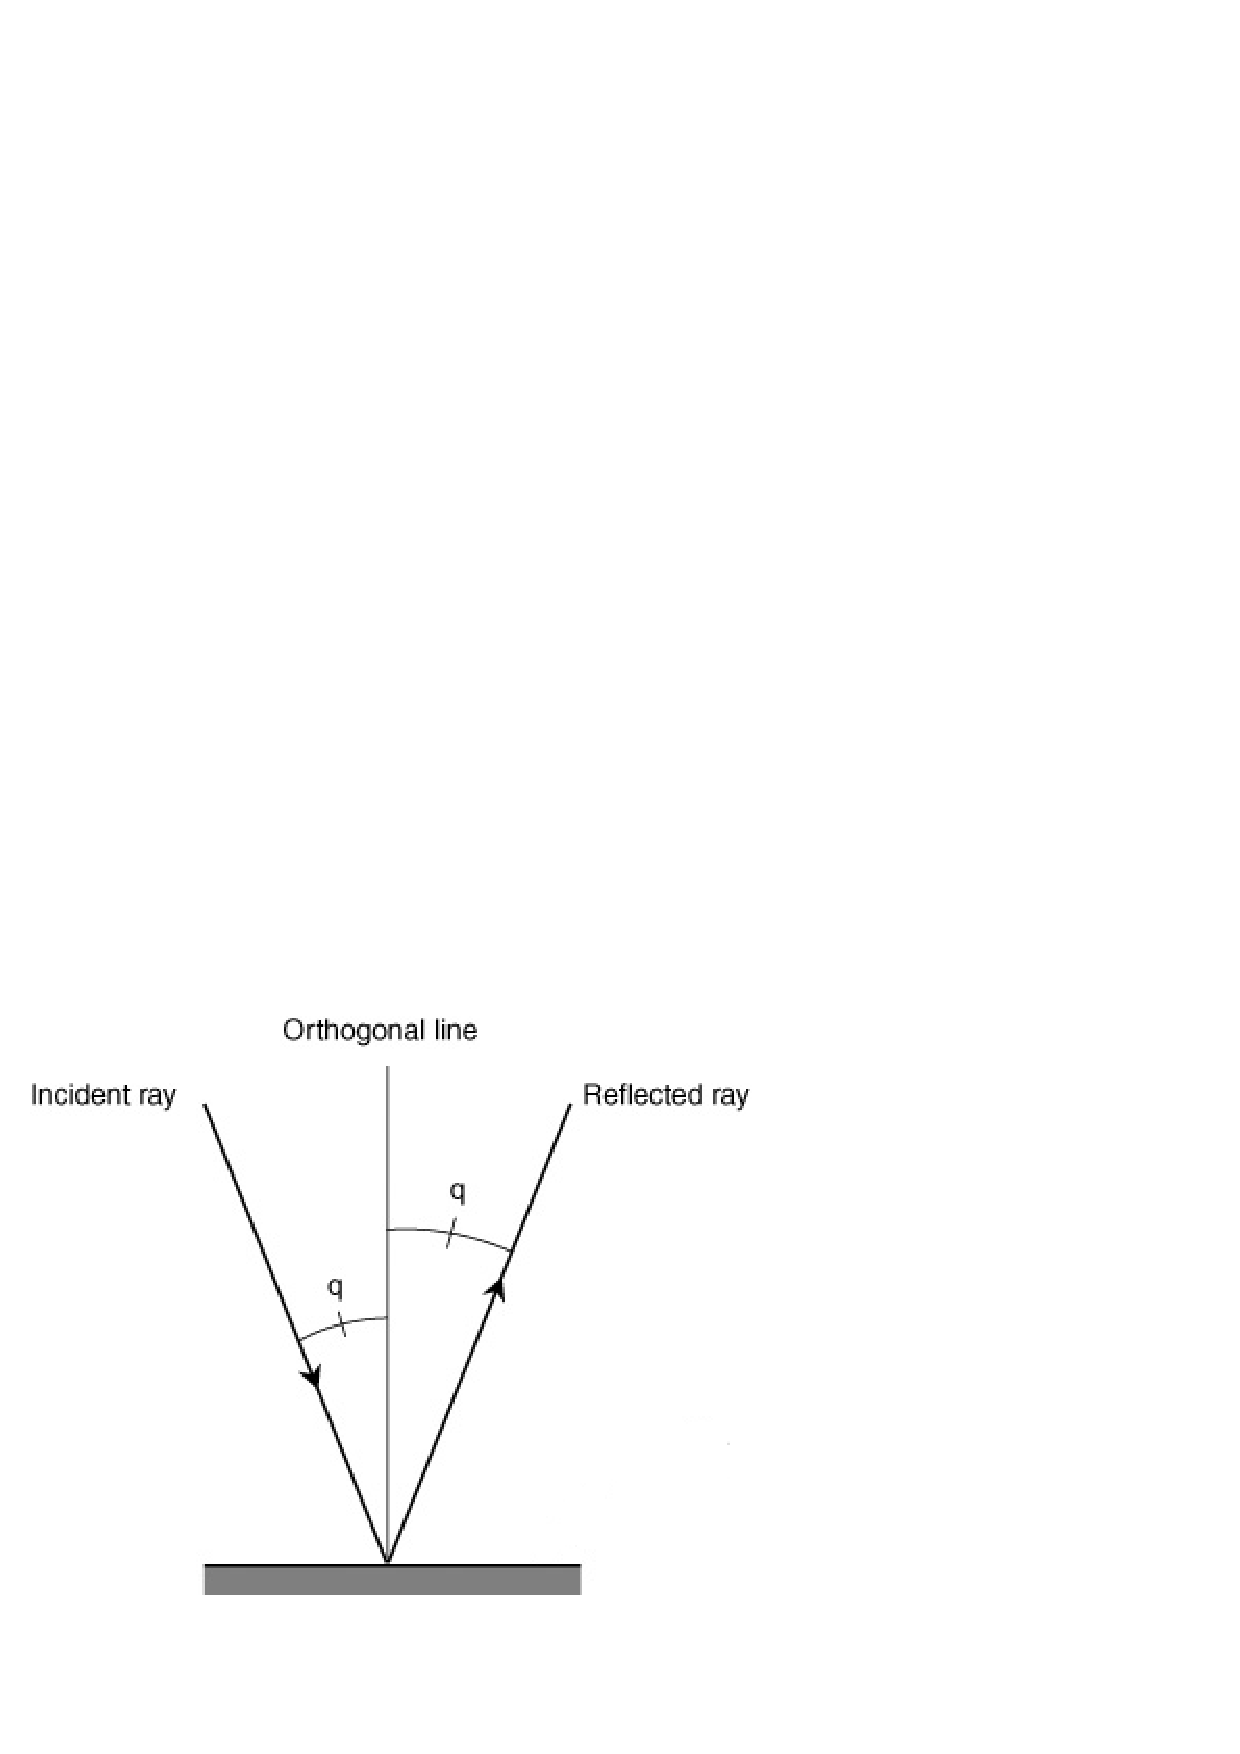
\includegraphics[width=2in]{particle_collision.png}
  \caption{\label{fig:collision-angle}Mechanics of a Billiard Ball Colliding with a Table Edge}
\end{figure}

Now, we shall label the horizontal sides of the table $h$ and the vertical sides of the table $v$. Whenever the billiard ball collides with a horizontal side (labelled $h$), we shall call the resulting collision an $h$-collision. Whenever the ball collides with a vertical side (labelled $v$), we shall call the resulting collision a $v$-collision.

We shall now define what this paper will be primarily interested in, a sequence of collisions:

\begin{definition}
  A \emph{collision sequence} ($\alpha$) is a sequence of $v$ and $h$ collisions which starts and ends with an $h$ collision for some ball $b$ with initial position $\bvec{x}_0$ and intial velocity $\bvec{v}_0$.
\end{definition}

Notice that all non-trivial initial conditions for a billiard ball will result in infinitely many $h$-collisions. The only initial conditions for which this is not true are when the initial velocity is parallel to the horizontal ($\bvec{v}_0 = (1, 0)$) so that the ball bounces infinitely between the two vertical sides. The proof of this is trivial and should become clear once the tiling representation is presented, so we will omit it.

Thus, it is perfectly reasonable to constrain a ball's collision sequence to begin and end with an $h$ collision, since one simply needs to extend the number of collisions one watches until the sequence of collisions begins and ends with an $h$-collision. This constraint will later make it easier to reason about properties of sequences.
